\documentclass[a4paper, 12pt]{article}
\usepackage[utf8]{inputenc}
\usepackage{geometry}
\usepackage{polski}
\usepackage{graphicx}
\usepackage{float}
\usepackage{etoolbox,refcount}
\usepackage{multicol}
\usepackage{tabularx}

\newgeometry{left=2cm, right=2cm, bottom=2cm, top=1.5cm}

\begin{document}
	\begin{figure}[H]
		\centering
		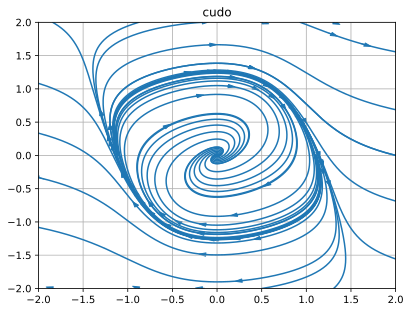
\includegraphics[width = \textwidth]{./img/cudo.png}
	\end{figure}
	\section{Cel ćwiczenia}
		Celem ćwiczenia jest zbadanie własności ruchowych silnika skoskowego reluktancyjnego, indentyfikacja parametrów przyjętego modelu silnika oraz weryfikacja praktycznej przydatności modelu na drodze porównania wybranych wyników symulacyjnych z odpowiednimi wynikami pomiarowymi.
	\section{Wprowadzenie}
		\begin{figure}[H]
			\centering
			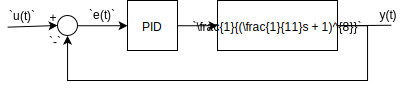
\includegraphics[width = 0.9\textwidth]{./img/schemat.png}
			\caption{Schemat układu}
		\end{figure} \noindent
		W ćwiczeniu mamy do czynienia z silnikiem skokowym reluktancyjnym typu LD20ACM-25. $T_N = 0.247 \mathrm{Nm}$, $I_N = 1.4 \mathrm{A}$, $U_N = 28 \mathrm{V}$, $R_{pasma} = 20 \mathrm{\Omega}$, skok $15^\mathrm{o}$, $J = 3,2\cdot10^{-6}\mathrm{kgm^2}$.
	\section{Przeprowadzenie ćwiczenia}
		\subsection{Maksymalna częstotliwość rozruchowa}
			Przy badaniu maksymalnej częstotliwości rozruchowej uruchamialiśmy silnik z zadaną przez nas częstotliwością, obserwując, czy nie gubi po drodze kroków. Po kilku próbach otrzymaliśmy wartości graniczne zarówno dla pracy całoskokowej jak i półskokowej:
			\begin{itemize}
				\item[--] półskokowa -- 34 Hz
				\item[--] całoskokowa -- 102 Hz
			\end{itemize}
		\subsection{Przebiegi}
			\subsubsection{Pomiary}
				Poniższy przebieg przedstawia zależność prądu od czasu dla silnika półskokowego. Różnica pomiędzy przebiegiem dla silnika półskokowego oraz całoskokowego polega na tym, że silnik półskokowy musi mieć dodatkowo prąd, który trzymałby wirnik w pozycji między skokami.
				\begin{figure}[H]
					\centering
					\includegraphics[width = 0.85\textwidth]{./pomiary/przebiegi.png}
				\end{figure} \newpage \noindent
				Poniższy przebieg przedstawia zależność prądu w zależności od czasu. Na podstawie przebiegu możemy stwierdzić, że jest to obiekt inercyjny I rzędu. Kreśląc styczną w miejscu, gdzie następuje zmiana wartości pozwala nam na wyznaczenie stałej czasowej $T=0,02\,\mathrm{s}$. Nie jest to jednak wartość dokładna, ze względu na drobne nierówności z początku.
				\begin{figure}[H]
					\centering
					\includegraphics[width = 0.85\textwidth]{./pomiary/hopniecie_inercja.png}
				\end{figure} \noindent
				Przebieg czasowy kąta obrotu silnika:
				\begin{figure}[H]
					\centering
					\includegraphics[width = 0.85\textwidth]{./pomiary/kat_od_czasu.png}
				\end{figure} \noindent
				Powiększony przebieg czasowy kąta obrotu silnika:
				\begin{figure}[H]
					\centering
					\includegraphics[width = \textwidth]{./pomiary/kat_od_czasu_blizej.png}
				\end{figure} \noindent
				Na powyższym przebiegu można zauważyć pojedyńcze skoki, które wykonuje silnik w trakcie pracy. Taka zmiana położenia sprawia, że silnik sprawia wrażenie poruszania się ze stałą prędkością.
			\subsubsection{Symulacja}
				Jak można zauważyć na poniższym przebiegu symulacyjnym, silnik w rzeczywistości zachowuje się zgodnie z modelem rzeczywistym. Różnice wynikają z mniejszej częstotliwości próbkowania w przypadku przebiegu rzeczywistego. Charakterystyki mają inny kąt opadania.
				\begin{figure}[H]
					\centering
					\includegraphics[width = 0.85\textwidth]{./symulacyjne/kat_od_czasu.png}
				\end{figure} \noindent
				Poniższy przebieg symulacyjny przedstawia zależność momentu od czasu. Ze względu na duże zmiany momentu siły silniki skokowe nie nadają się do wielu zastosowań.
				\begin{figure}[H]
					\centering
					\includegraphics[width = 0.85\textwidth]{./symulacyjne/moment_od_czasu.png}
				\end{figure} \noindent
				Poniższy przebieg symulacyjny przedstawia zależność poboru prądu w zależności od czasu. 
				\begin{figure}[H]
					\centering
					\includegraphics[width = 0.85\textwidth]{./symulacyjne/prad_od_czasu.png}
				\end{figure} \newpage \noindent
				Poniższy wykres przedstawia uzyskaną w symulacji statyczną zależność momentu postojowego silnika od kąta wychylenia wirnika. Do symulacji podaliśmy jako argumenty wartości, kątów oraz momentów, które wyznaczyliśmy doświadczalnie.
				\begin{figure}[H]
					\centering
					\includegraphics[width = 0.85\textwidth]{./symulacyjne/moment_od_kata.png}
				\end{figure}
		\subsection{Rezystancja}
			Po wykonaniu ćwiczenia, gdy silnik był częściowo nagrzany mogliśmy zmierzyć rezystancję nagrzanego uzwojenia oraz rezystancję uzwojenia zimnego. Dokonaliśmy tego mierząc napięcie na uzwojeniu oraz przepływający przezeń prąd. Następnie skorzystaliśmy z prawa Oma:
			\begin{itemize}
				\item[--] $R_{n} = \frac{U}{I} = 24\mathrm{\Omega}$ -- nagrzany
				\item[--] $R_{c} = \frac{U}{I} = 23,67\mathrm{\Omega}$ -- zimny
			\end{itemize}
	\section{Wnioski}
		Ćwiczenie te pozwoliło nam na zapoznanie się z silnikami krokowymi. Dowiedzieliśmy się jak w rzeczywistości wyglądają ich przebiegi oraz momenty w zależności od kąta.
		\newline 
		\newline 
		Dowiedzieliśmy się na jakiej zasadzie dokonuje się rozruch takiego silnika oraz co się dzieje w przypadku zasilania większymi częstotliwościami od maksymalnej częstotliwości rozruchowej. Zobaczyliśmy w praktyce jak wygląda gubienie skoków przez taki silnik.
		\newline 
		\newline 
		W trakcie wykonywania ćwiczenia zobaczyliśmy jak w praktyce wyglądają przebiegi prądów poszczególnych uzwojeń w przypadku pracy całoskokowej i półskokowej oraz jesteśmy w stanie je rozróżnić.
\end{document}